\chapter{Background}
\label{background}

This chapter summarises research related to PrologPF, in the areas of
parallel Prolog, functional logic, and the prior work on the
Delphi machine.

PrologPF is an or-parallel implementation of Prolog
on the Delphi machine without \textit{cut},
\textit{assert} or \textit{retract}.
The language has been extended with the definition and deterministic evaluation
of higher-order functions, and the review of related research in this 
chapter reflects these design choices.

%%%%%%%%%%%%%%%%%%%%%%%%%%%%%%%%%
\section{Parallelism in Prolog} %
%%%%%%%%%%%%%%%%%%%%%%%%%%%%%%%%%

\todo{more references in this section}

As discussed in Chapter \ref{intro}, a pure Prolog program can be
parallelised by:
\begin{itemize}
\item{parallel selection of clauses to prove subgoals}
\item{parallel execution of subgoals in the body of a clause}
\item{parallelisation of the unification of multiple or compound arguments}
\end{itemize}

These forms of parallelism are \textit{or-parallelism}, \textit{and-parallelism}
and \textit{unification parallelism} respectively.

Or-parallelism is illustrated in the proof tree of figure \ref{or_parallelism}, where
the dashed lines surround the subtrees of the proof tree which can be searched in
parallel.  The conjunctive subgoals \texttt{p(U), q(V), r(U,V)} may still be
executed sequentially, but the clauses forming the procedures for \texttt{p} and
\texttt{q} may be searched in parallel.

\begin{figure}[h]
\vspace{5mm} \hbox to \hsize{\hfill \psfig{file={background/ps/or_parallelism.ps}} \hfill}
\caption{Or-parallel execution of goal clause g(U,V).}
\vspace{5mm}
\label{or_parallelism}
\end{figure}

Similarly, and-parallelism is illustrated in figure \ref{and_parallelism}, where
the subgoals \texttt{p(U)}, \texttt{q(V)} and \texttt{r(U,V)} can be solved in
parallel.  Support is required to communicate bindings of shared variables
between subgoals.

\begin{figure}[h]
\vspace{5mm} \hbox to \hsize{\hfill \psfig{file={background/ps/and_parallelism.ps}} \hfill}
\caption{And-parallel execution of goal clause g(U,V).}
\vspace{5mm}
\label{and_parallelism}
\end{figure}

Systems supporting \textit{and-or} parallelism would combine the approaches of
figures \ref{or_parallelism} and \ref{and_parallelism} such that all five
dashed areas in figure \ref{or_parallelism} could be searched concurrently.

The attempted proof of each subgoal involves the unification of the arguments
in the subgoal with the arguments given in each clause of the defining
procedure. For example, the arguments \texttt{U,V} of the subgoal \texttt{r(U,V)}
will be unified with the arguments \texttt{X,X} in the fact defining \texttt{r}.
In general, the multiple arguments may be unified concurrently, and the
unification algorithm itself contains opportunities for parallel execution when
compund terms (such as \texttt{a(b,X,c(Y))} and \texttt{a(Z,b,c(d))}) are
unified.  Few systems have exploited the potential concurrency in unification,
and the technique is not used in PrologPF.  Unification concurrency will not be
discussed further in this dissertation.

\subsection{Or-parallelism}
%%%%%%%%%%%%

The or-parallel search of alternate clauses takes place in the context of
the variable bindings arising from the search leading to the current choice point.
The issue is shown best with the transformed or-only tree. 
The shaded areas in figure \ref{or_context}
show the subtrees for \texttt{q(V)} for or-parallel search, in an environment
where \texttt{p(U)} has already provided the binding \texttt{\{U/1\}}.

\begin{figure}[h]
\vspace{5mm} \hbox to \hsize{\hfill \psfig{file={background/ps/or_context.ps}} \hfill}
\caption{Variable bindings in or-parallel subtrees.}
\vspace{5mm}
\label{or_context}
\end{figure}

A subgoal \texttt{r(U,V)} appears in each shaded area, the first of which 
contains the binding \texttt{\{U/1\}} from the earlier search and \texttt{\{V/1\}}
from the chosen solution for \texttt{q(V)}.  \texttt{r(U,V)} in
the second shaded area will be searched in the context
\texttt{\{U/1,V/2\}}.

Thus with or-parallel execution the system must ensure that the search continues
in the context of the current variable bindings, and that new bindings arising in
the or-parallel subtree must be limited in scope to that search.

Three techniques are commonly used to propagate and limit the scope of variable
bindings in or-parallel systems:
\begin{enumerate}
\item{The shared-binding environment model: a data structure is maintained in
  memory representing the tree structured binding hierarchy as the search is
  executed, with each processor building their new bindings and referencing
  existing bindings higher up the structure.  This model is better suited to
  shared memory computers \cite{DR92}.}
\item{The closed environment family: at each choice point for or-parallel
  execution the environment is copied to each selected processor, which
  continues by locally extending that context.  This technique is suitable for
  distributed implementation if communications can be minimised, for example
  by using broadcast to propagate the environment to many processors}
\item{The recomputation family: the search path to a given choice point for
  or-parallel execution is recomputed by the selected processors, such that
  the environment at that choice point is rebuilt locally in each processor.
  This technique is suitable for systems with high communications overhead.}
\end{enumerate}

The techniques listed above show fundamental design choices in the implementation
of the work splitting method.  With any of these methods the scheduling
\textit{strategy}
used to decide at which point the problem should be divided is as
important as the technique used to communicate the task.
The most simplistic strategy might be to divide the work at every choice point, to
as many processors as there are alternate clauses.  However, more efficient
execution with better load balancing will generally be achieved with more sophisticated
strategies \cite{Sar95, AKM91, Bea91}.

PrologPF provides or-parallelism through recomputation, and the underlying
priciples and related research are covered in a separate section,
\ref{delphi_machine_pwork}.

\subsubsection{Muse}

Muse \cite{AKM91}
is named after \textbf{Mu}lti-\textbf{Se}quential Prolog Engines and is
a development of the Multi-Sequential Machine \cite{Ali87}.
The system supports or-parallel execution of full Prolog, with each processor having
access to local and shared memory. 
During execution, the or-nodes representing the choice points in the
search can be either \textit{private} or \textit{shared}.
Private nodes are accessible only by the worker which created them.
Shared nodes are accessible to all workers searching a subtree beneath that
node. Work is divided between worker processors by
moving the previous or-nodes from the private area to the shared area, and
incremental copying of the WAM stack (the trail) to the new worker.

The target architecture for the Multi-Sequential machine supported limited
broadcast to local memory of each worker \cite{Ali88},
so the overhead of copying the WAM
stacks to multiple workers was minimised.  Muse has been implemented on
parallel computers with both broadcast and switched communications support.

The scheduling strategy used in Muse attempts to reduce the overhead of
work allocation, with the incremental copying of WAM stacks to new workers
and the assignment of multiple choice points to a new worker.

Muse is implemented upon sequential SICStus Prolog \cite{BBP+94}, and has been shown to
have a higher speedup than Aurora (see below) for the same benchmarks
\cite{AKM91}.

\subsubsection{Aurora}

%\ todo{Kacksuk and Wise p. 22, Proc 5th Intl Conf LP p.1531..1545}

Aurora \cite{LWH+90} is a prototype or-parallel implementation of Prolog for
shared memory multi-processors based on the SRI model \cite{War87}.
It supports the full Prolog language,
thus being able to execute existing Prolog programs without any change.
The system was a joint project between Argonne National Laboratories,
Universty of Bristol, and the Swedish Institute of Computer Science.

Aurora uses a storage model in which the path of the search is represented
by a group of intertwining WAM stacks \cite{Tic91}, with a stack group allocated
to each processor.  Each choice points creates a branchpoint on the stack, and
an idle processor can form a branch of the or-tree emanating from that branchpoint.
Holes may form in the stack groups when a branch ``dies back'', i.e. when
backtracking fails through the branchpoints of the branch.  However, that 
stack group may have been extended with another independent branch, and garbage
collection will be delayed until the covering branch is completed.

In searching the branches from that choice point, multiple processors can
produce independent solutions, i.e. different but valid variable bindings.  Thus
bindings cannot be stored as values in the logical variables,  and a \textit{binding
array} is used per processor.  The binding array is essentially a software cache
of variables and their values, for exclusive use by the associated worker processor.

The Aurora systems is implemented using SICStus Prolog \cite{BBP+94} and has
provided a platform for the evaluation of multiple scheduling strategies
\cite{Bea91}.  The scheduler determines how tasks should be allocated to idle
worker processors and synchronises the access to the shared nodes nearer the
root of the search tree.

\subsubsection{Kabu-Wake}

%\ todo{ref sanjay, Kacsuk and Wise p.24}

The Kabu-Wake model \cite{MKI+86}
is based upon environment copying with selective backtracking
to allow processors to compute alternate paths.

A processor computes sequentially until it is interrupted with a request for
work from an idle processor.  The busy processor (called the \textit{parent}) suspends
its computing when the request is received, sends a copy of its environment to the
idle processor, and then resumes.  Part of the splitting procedure requires the
parent to temporarily backtrack to the splitting choice point, so that the more
recent variable bindings from the choice point are undone.  In order to recognise
the validity of the bindings, the system uses an incremental timestamp in each
variable cell.

The model leaves open the
specification of the algorithm for the selection of a suitable parent
by an idle processor.
The response of a parent to an interruption is immediate, without
optimisations to improve the task granularity.
Load balancing is performed by the selection of the parent
processors by those which are idle.  Efficient performance would require the copying
be minimised by targeting problems with well balanced search spaces \cite{DR92}.

%\ todo{comment in Kacsuk and Wise p.24, sanjay p.12}

\subsubsection{OPERA}

The OPERA project \cite{B+92} was inspired by the Kabu-Wake model (see above) with the
principle that the complete state of a busy processor is transferred to an idle one
to effect work sharing.  The target architecture is similarly distributed processors with
a high-performance communications network providing node-to-node connectivity.  The
implementation of OPERA on a dynamically reconfigurable array of Transputers is optimised
for a system with relatively long connection setup times ($\geq\ 250\ \mu s$) but an
efficient matrix block tranfer performance. Each point-to-point connection can tranfer
data at between 500Kbps and 1Mbps (b=byte).  DMA is used (Direct Memory Access) to move
the data into and out of the processor memory so that processing can continue concurrently.
Most importantly, a crossbar switch system is used to implement the network so that many
transfers can take place in the network concurrently.  The relatively long communications
setup time means that short data transfers are relatively inefficient, precluding the
use of stack sharing models as in Aurora (see above).

A multi-sequential approach is used: each processor executes a complete Prolog engine based
upon an extended WAM.  The stack data structures are modified to improve the
efficiency of the copying operation.
Choice points are managed in a separate double-linked list,  rather than
being intertwined with the clause activation records as in a standard WAM.  This separation is
similar to the technique used in Muse (see above), and improves the efficiency of work splitting.
Variable bindings on the trail stack are timestamped.  Work splitting at a given choice point
would require all variable bindings that had occurred after that choice point be unbound.  The
timestamps (as in the Kabu-Wake model) mean that the copy process need not thread though the
trail stack to unbind these variables, but can simply compare the timestamp with that of
the choicepoint.  To minimise further the amount of stack copying, the prototype always splits
with work of an active worker at the topmost choice point (i.e. nearest the root), such that the
stacks to this point are as short as possible.

As the cost of task creation on an idle processor is relatively high, involving the copying
of the state of the active processor,  scheduling in OPERA is important \cite{B+92}.
The scheduler has to consider the export and import time of the active and idle processors compared
to the expected time for the search of the current subtree to complete.  The scheduler should
ensure that the active worker, in passing choice points to an idle worker, keeps enough work
to remain active after the initialisation of the new task.  After consideration of alternatives,
a scheduling model with a hierarchy of scheduling processes was used, with \textit{spy} processes
on each worker processor to estimate the workload of the active workers.  The workload 
estimate is performed dynamically, with the simple heuristic being used of the number of
choice points being held by the worker.

Good speedups have been achieved with the prototype up to a maximum of 16 processors.
Further developments are aimed at reducing the task creation overhead through the use of
incremental copying.

%\ todo{ref Kacsuk and Wise Ch. 3 - good paper}

\subsubsection{ANL-WAM}

%\ todo{ref DLO87 in Proc 4th Int Conf on LP V2- original paper}

The ANL-WAM was an early experimental implementation of or-parallel Prolog 
at Argonne National Laboratory on a
shared-memory multiprocessor (a 20-cpu Encore Multimax).
The principles evaluated using this system \cite{DLO87} were used in the subsequent development
of Aurora (see above).

As with Aurora, a hash-table structure was used to cache the multiple variable bindings
arising from or-parallel execution of alternate choice points.  With ANL-WAM,
starting a new worker process involves giving the worker access to the variable bindings
created so far, and the creation of a new hash table to store the new variable bindings
resulting from the allocated branch.  As shared memory was used, the copying process could
be limited to the headers of the hash table with pointers to the existing shared nodes.
The allocation of work to new workers was thus efficient, with the design decision taken to
trade this against contention for subsequent access to shared variables.

The scheduling algorithm used in ANL-WAM created a fixed number of worker processes to
be assigned to branch points as they were created.  On finishing a branch, the process will
seek more work to do from a dispatching pool.  A graphical display tool was created to play
back a trace log showing the growth of the search tree and the allocation of branches to
worker processes.  The tool was used to improve the dispatching algorithm.

Results were produced from ANL-WAM \cite{DLO87}, showing effective speedups for some problems
up to a maximum of 16 worker processes.

\subsubsection{Boplog}

%\ todo{ref TL87 p.601 in Proc 4th Int Conf Logic Prog - orig paper.  Kacsuk Wise p.13}

Boplog \cite{TL87}  is a multi-sequential or-parallel Prolog design
implemented on the BBN Butterfly Parallel Processor, which is a multi-cpu
shared memory design.  The memory consists of segments local to each processor, which can
be accessed remotely by all other processors.  Each processor's address space is
defined locally, such that an address of a word on a remote cpu may be different to
different processors.  The Boplog
implementation attempts to optimise the use of the segmented memory.

To support parallel execution, the design 
makes extensive use of shared data structures rather that structure copying, as the
non-local memory access time ($6.3 \mu$s) was considered reasonably fast compared to the
local memory access time of $1.35\mu$s.  The resulting slower access time to shared data
and less efficient reclamation of heap and stack space, which cannot be released until no other
processors need access to it, are traded for less time for copying and less memory for
redundant or unused data \cite{TL87}.

In Boplog, variable bindings are timestamped and stored in a doubly-linked list to
improve the efficiency of the work reassignment.  Scheduling is achieved by idle processes
obtaining more work from busy processes, selecting the untried branch nearest the
root of the search tree.  The early analysis of Boplog's runtime behaviour suggested that
work was reassigned on average every millisecond, with the allocation typically involving the
transfer of 100 bytes of data.

\subsection{And-parallelism}
%%%%%%%%%%%%
\label{and_parallelism_section}

%\ todo{ref intro in Takeuchi Parallel Logic Programming}

With the AND-parallel execution of a Prolog Program, the conjuctive subgoals in the
body of a clause are solved concurrently, while the alternative clauses in a
procedure are tried sequentially. According to the handling of shared variables,
the model can be further divided as follows \cite{CK81}:
\begin{description}
\item[Independent AND-parallelism:]{ Even when the subgoals share variables
  they are solved independently.  After all solutions are found, the shared
  variables are tested for consistency.}
\item[Dependent AND-parallelism:]{ Also called stream-and parallelism, subgoals
  with shared variables are executed dependently, that is they interfere with
  one another.  The word \textit{stream} is used to represent the flow of bindings
  from one and-parallel process to another.}
\item[Restricted AND-parallelism:]{ Subgoals sharing no variables are executed in
  parallel, while subgoals sharing variables are executed sequentially.}
\end{description}

The communication of solutions (i.e. variable bindings) between and-parallel
subgoals is illustrated in figure \ref{stream} where the three subgoals for
\texttt{p}, \texttt{q} and \texttt{r} are
represented by the processes A, B, and C respectively.

\begin{figure}[h]
\vspace{5mm} \hbox to \hsize{\hfill \psfig{file={background/ps/stream.ps}} \hfill}
\caption{Communication of bindings in dependent and-parallelism.}
\vspace{5mm}
\label{stream}
\end{figure}

The following sections summarise implementations of the and-parallel logic computation
model.  PrologPF is based upon the purely or-parallel Delphi machine, but an effort
to extend the machine to support both and- and or-parallel execution \cite{Wre90}
is summarised in section \ref{delphi_machine_pwork}.

\subsubsection{Parlog}

%\ todo{comments in Wise p. 94, paper in Shapiro V1 p.84}

Parlog is a stream and-parallel logic programming system in which the logic
variables can be thought of as channels, down which partial results are sent between
literals that are executed in parallel \cite{CG84}.  The model is suited to
implementation on a dataflow archicture computer, or a conventional multiprocessor
with shared memory.

The language implemented in Parlog is that of guarded Horn clauses, built upon the
syntax and semantics developed in \cite{CG81}.  Procedures are annoted with \textit{mode}
information, specifying which logical variables should be inputs and outputs to each
procedure. The \textit{guards} are goals added to each clause so that the form of
clause selection is \textit{committed choice}, i.e. only one clause will be selected for
which the guard literals evaluate to \textit{true}.  Parlog will only ever find one
solution to a query.
At the time of the parallel guard evaluation, all guard literals must be
\textit{ground}, i.e. contain no variables.  Both serial and parallel forms
of connectives can be used in the definition of the goal sequence in the body of 
a clause. ``\texttt{\&}'' implies sequential left-to-right execution of the goals, while
``\texttt{,}'' implies the goals can be executed in parallel.  A later extension to
Parlog allowed similar annotation of the clauses in a procedure, where ``\texttt{.}'' 
permits or-parallel search, while ``\texttt{;}'' implies top-down sequential search.

The treatment of variables in Parlog in optimised for stream and-parallelism, with
the \textit{don't care} parallelism (i.e. the commitment to the first goal with a
successful guard) limited to committed choice non-determinism.  The or-parallel
execution is provided though all-solution operational model using set expressions.

\subsubsection{Concurrent Prolog}

%\ todo{ref Shapiro, Wise p. 108}

Like Parlog, Concurrent Prolog in based upon the stream and-parallel model and
associated committed choice language proposed in \cite{CG81}.  The system has
been simulated in Prolog, with the proposal that it is best suited to multiprocesor
dataflow architecture machines \cite{Sha87a}.

Concurrent Prolog does not require the guard literals to be ground at the time of
evaluation, such that clause selection (and commitment) does not just rely upon
successful evaluation of the guard sequence as in Parlog.  The evaluation of the
guards must also return a set of variable bindings.

The committed choice nature of the clause selection, with the resultant single solution to
each goal, means that for many general logic programs the system may fail to
find a solutions.  For example \cite{Wis86},
\begin{verbatim}
simple(X) :- p(X),q(X).
p(1).
p(2).
q(1).
q(2).
\end{verbatim}
The Concurrent Prolog query \texttt{solve(simple(X))} may commit to the solution
\texttt{X=1} for \texttt{p(X)} and subsequently fail the goal \texttt{q(X)}.

In a nutshell, both Parlog and Concurrent Prolog have adopted a semantics markedly
different than that of sequential Prolog.

\subsubsection{Delta Prolog}

%\ todo{comments in Wise p. 115, [CMCP92] paper in Kacsuk and Wise}

Delta Prolog is a logic programming language extending Prolog with constructs for
sequential an parallel composition of goals, interprocess communication and
synchronisation, and external non-determinism \cite{CMCP92}.  The language is
optimised for execution on distributed machines, and makes extensive use of the
concepts of Communicating Sequential Processes (CSP) \cite{Hoa85}.

As with CSP, parallelism is made explicit in Delta Prolog through the use of a 
\textit{split} operator \texttt{//} where goals \texttt{S$_1$//S$_2$} are to be
evaluated in parallel.  Channels for communication between goals are established 
though the use of \textit{event goals}, with \texttt{X!chan} being considered to
send the value of \texttt{X} along channel \texttt{chan}, to be received by a
complimentary subgoal \texttt{Y?chan} in a concurrently executed goal.  To be an
acceptable candidate to receive the value, the 
arbitrary terms \texttt{X} and \texttt{Y} must
be unifiable, and the atom naming the channel the same in both the transmitting and
receiving event goals.
The event goals can be \textit{guarded} though the use of associated goal sequences
with the syntax \texttt{X?chan:G} where \texttt{G} is the goal sequence which must
evaluate to \texttt{true} for the communication event to be accepted.  Non-deterministic
acceptance of a communication event is provided though the definition of \textit{choice
goals}.  These goals have the form \texttt{A$_1$::A$_2$::\ldots::A$_n$} where each
\texttt{A$_i$} is of the form \texttt{H,B} with \texttt{H} an event goal and \texttt{B}
the (possibly empty) body of the alternative clause.

The system provides efficient support for the communication of values though the
use of event goals.  Non-deterministic evaluation of goals requires the implementation
of distributed backtracking.  The prototype implementation  supports backtracking in
some simple programs, but this is an area of ongoing research.

\subsubsection{EPILOG}

%\ todo{ref Wise [Wis86]}

EPILOG is wholly based upon the dataflow model of computation \cite{Wis86}.  In
place of Prolog's depth-first, left-to-right evaluation strategy, the EPILOG model,
by default, evaluates all clause-body literals in parallel, that is performs
breadth-first execution.  All solutions to a query are found in parallel, and
\textit{back-unification} (the propagation of unifiers from subgoals back up to higher
level goals) is used to be \textit{equijoined} with other partial solutions to be
propagated to still higher level goals.

The process is illustrated for the query \texttt{ans(X,Y,Z)} in figure \ref{epilog}.

\begin{figure}[h]
\vspace{5mm} \hbox to \hsize{\hfill \psfig{file={background/ps/epilog.ps}} \hfill}
\caption{Dataflow communication of bindings in EPILOG.}
\vspace{5mm}
\label{epilog}
\end{figure}

EPILOG would be
overwhelmed with data
Without mechanisms to reduce the combinatorial explosion of data transfers arising from
the breadth-first nature of the parallel execution.  Fixed sequencing constructs are
provided to reintroduce left-to-right evaluation of clause-body literals and to
order the clauses in a procedure.  In addition, \textit{mode} information on variables
can be specified, and \textit{thresholds} can be specified giving the number of
arguments to be ground before a clause will be executed.

\subsection{Other forms of parallelism in Prolog}
%%%%%%%%%%%%

As was mentioned in Chapter \ref{intro}, the unification algorithm used in Prolog 
to match a subgoal with a suitable clause head contains opportunities for
parallel execution.

\begin{description}
\item[Parallel unification of multiple arguments:]{ With a subgoal \texttt{p(a,b,c)} and
  a clause \texttt{p(X,Y,Z) :- \ldots} each argument can be unified in parallel, arriving at
  the unifier \texttt{X/a,Y/b,Z/c}.  Where variables are repeated in the clause head,
  a communication mechansim must be provided to synchronise the shared binding.}
\item[Parallel unification of compound subterms:]{ Each argument to a relation may be 
  a compound term with a tree internal representation.  Different branches of the
  tree may be unified in parallel with corresponding elements of the argument in the
  clause head.  This technique is a generalisation of the one given above.}
\end{description}

Effort into the concurrent execution of the unification algorithm has been limited, and
in PrologPF and other or-parallel Prolog systems the unification algorithm is 
sequential.

%%%%%%%%%%%%%%%%%%%%%%%%%%%%
\section{Functional Logic} %
%%%%%%%%%%%%%%%%%%%%%%%%%%%%

The integration of functional and logic programming languages can be approached from either
a functional or logical starting point although both techniques lead to similar
operational principles (\cite{Han94}).  As the primary fondation for PrologPF is
logic programming, the existing research listed here been selected with that approach.

A survey of the field giving an introduction to the alternative approaches can be found
in \cite{BL86}, and a more recent summary with an emphasis on narrowing \cite{Red85} with
application specific abstract machines can be found in \cite{Han94}.

\subsection{Functions as deterministic Prolog procedures}
%%%%%%%%%%%%
\label{det_procs}

The eager evaluation of a function of $N$ arguments can be replaced with the
execution of a Prolog goal of $N+1$ arguments,
where the additional argument is a logical variable to hold the
result.  For example the function \texttt{factorial(N)} can be
replaced with the relation \texttt{factorial(N,F)}:
\begin{verbatim}
factorial(1,1).
factorial(N,F) :- N > 1,
                  N1 is N - 1,
                  factorial(N1,F1),
                  F is N * F1.
\end{verbatim}
The advantage of this approach is that the simple syntax and semantics of standard
Prolog can be retained for functional programming as well as non-deterministic logical
programming for which Prolog was designed.  The disadvantages include:
\begin{enumerate}
\item{\textbf{Higher-order functional programming:}  functions are not treated as
  first-class data items in Prolog.  For higher-order application of functions the
  programmer must adhere to arbitrary programming conventions and use meta-logical
  relations such as \texttt{call} to use functions as arguments and results.  Effort
  has been applied to retaining the relational definitions of functions but adding
  higher-order support to Prolog, particularly through the use of \texttt{call/N}
  \cite{SHC95,Nai96} and \texttt{apply/3} \cite{Nai96}.  These techniques are
  compared with PrologPF in Chapter \ref{functions}.}
\item{\textbf{Flat programming style:} the flat syntax of standard Prolog means that
  all intermediate functional results must be given a name.  This requirement has
  been likened to assembler \cite{App92}.  To reduce the problem, Prolog supports
  nested arithmetic expressions as the second argument to the special \texttt{is}
  relation, but this support is arbitrarily limited to this special use.}
\item{\textbf{Use of \textit{cut}:} The deterministic evaluation of functions typically
  requires the use of guard conditions in the definition of the alternate clauses in the
  Prolog procedure (see \texttt{N > 1} in \texttt{factorial} example above).  For a
  procedure with many clauses, the guard conditions can become unwieldy, such that the
  use of \textit{cut} simplifies the definition of the sequential algorithm, excluding
  subsequent clauses from providing alternative solutions.  The use of \textit{cut}
  introduces considerable complexity in the or-parallel execution of Prolog programs.
  The issue is covered in detail in Chapter \ref{cut}.}
\item{\textbf{Execution efficiency:} the execution model for
  the deterministic eager evaluation of functions lends itself to efficient implementation
  compared to the unification and backtracking requirements of a Prolog program.  The
  compile-time analysis of logic programs to recognise deterministic modes of execution
  is a topic of current research in systems such as Mercury \cite{HCSR95}.  The use of
  \textit{cut} does not imply determinacy (see Chapter \ref{cut}).  Use of a syntax 
  for functions other than that of standard Prolog can render explicit the requirement for
  deterministic evaluation.}
\end{enumerate}

\subsection{Term evaluation}
%%%%%%%%%%%%

The most straightforward approach to adding functions to Prolog is to require the arguments
to be fully instantiated before reduction is attempted.  The operational semantics of Prolog
can be maintained and the responsibility for this requirement placed on the programmer, e.g. in
the standard \textit{is} predicate.  Alternatively,
function evaluation can be deferred until this condition is met.
This technique is called \textit{residuation}, see \cite{AKLN87}.

A simple example may illustrate the principle, from \cite{MBB+93}:

\noindent
%_ \hrulefill
\begin{verbatim}
		length([], 0).
		length([X|Xs], N + 1) :- length(Xs, N).

		:- length([a,b,c], 5).
		no

		:- length([a,b,c,d,e], 5).
		yes

		:- length([a,b,c], L).
		L = 3

		:- length(List, 5).
		List = [_,_,_,_,_]

		:- length(List, L).
		List = [], L = 0;
		List = [_], L = 1;
		List = [_,_], L = 2;...
\end{verbatim}
%_ \hrulefill

In the above example, \texttt{N + 1} is a functional term providing a natural expression
of the problem with more generality than that provided by \textit{is}.
This is illustrated by the last two examples, where with the Prolog operational semantics
non-ground functional terms (i.e. $N + 1$) will be encountered during execution.  In implementations
providing residuation (e.g. Le Fun \cite{AKLN87}, GAPLog \cite{MBB+93}),
the function call (+) will be delayed.  In the case of arithmetic, unification of 
two terms $t_1, t_2$ reduces to solving the equation $t_1 = t_2$. If further constraints are
imposed upon the arguments, namely (\cite{MBB+93}):
\begin{itemize}
\item{\textit{Equivalent arguments}. $t_1$ and $t_2$ are equivalent if and only if evaluation of
  all their ground subterms makes them identical, and unification succeeds with a null unifier.}
\item{\textit{$t_1$ or $t_2$ is a variable $X$.}  If the other term $t$ does not include $X$ (occurs
  check) then unification succeeds with the mgu $\theta = \{X/t\}$.}
\end{itemize}
then we approach the limitations of the predefined Prolog predicate \textit{is},
supporting calls such as
\texttt{X is 3 + 4} and \texttt{7 is 2 + 5}
\footnote{In fact with Prolog's \textit{is} 
  only the right-hand argument is evaluated, so \texttt{2 + 3 is 4 + 1} fails.
  The built-in arithmetic predicate '=:=' will evaluate the arithmetic 
  expressions on both the left-hand and right-hand sides, each side
  must be ground and \texttt{Z =:= 2 + 3} fails}.

Instantiated term evaluation allows external functional procedures to be used in Horn clauses,
and does not require the definition of the functions in a common language.  As the determinism of
the functions is explicit, the programs can be executed more efficiently than within the
general execution mechanism of the logic programming environment.

While residuation
ensures the function calls are only made when sufficiently instantiated, the procedure is
essentially incomplete and does not allow for function inversion.

\subsection{Mode and determinism declarations for relations}
%%%%%%%%%%%%
\label{modes}

Many Prologs include support for mode declarations for system and user defined relations,
for example the SISCtus list library relation to return the maximum member of
a list (\cite{BBP+94}):\\
\begin{center}\texttt{maxlist(+,?)}\end{center}
indicates that the first argument to \texttt{maxlist} must be fully
instantiated (i.e. ground) before the call,
and the second argument can contain zero or more variables
(i.e. be ground or non-ground).  Thus permitted calls include:\\
\begin{center}\texttt{maxlist([1,2,3],X)}\end{center}
which will succeed with the substitution \{\texttt{X/3}\} and\\
\begin{center}\texttt{maxlist([1,2,3],2)}\end{center}
which will fail.

The mode declaration provides an opportunity for the Prolog compiler to produce more efficient
code, as choice points can be eliminated and the unification of parameters need not be as
general.  Most implementations of Prolog (e.g. SICStus) perform \textit{no}
optimizations based on the mode statements provided by the programmer, and the information is
treated as a comment.

Other logic languges, in particular Mercury (\cite{SHC95}), make extensive use of the mode
information to generate efficient code.
In the Mercury syntax, the \texttt{maxlist} relation would have two modes:\\
\begin{center}\texttt{mode maxlist(in,out)} and \texttt{mode maxlist(in,in)}\end{center}
Note that for every mode of a predicate in which an argument is \textit{produced} (mapped
from free to bound) there is another mode for that predicate in which the argument is
\textit{consumed} (mapped from bound to bound), and similarly arguments ignored (mapped from
free to free) have another mode with the argument mapped from bound to bound.  These additional
modes are referred to in \cite{SHC95} as \textit{implied modes}.
In addition, Mercury can annotate mode declarations with their intended determinism, with tags of
\texttt{det, semidet, or nondet} to indicate that calls of the given mode have exactly one
solution, zero or one solutions, or zero to many solutions respectively.

The Mercury compilation process transforms a logic
program to C, and the current implementation \textit{generates separate code for each
declared and implied mode of each
predicate.}

This metalogical information enables the compiler to perform significant additional error
checking and to generate efficient code for each mode.  Inline code can be generated for some
relations and for certain instances of unification, for example instances of 
\texttt{X = Y} where one of X and Y is input (i.e. ground $\rightarrow$ ground) and the other is
output (free $\rightarrow$ ground).  Deterministic relations are transformed directly into C code for
an efficiency comparable with that of imperative languages, while relations with
the mode \textit{semidet}
are transformed into deterministic C code returning a success/fail indication.
Non-deterministic modes are supported with the simulation of a virtual machine similar to
the WAM \cite{AK90}.  Execution of some simple deterministic and nondeterministic benchmarks
(translated from Prolog) suggests an improvement in efficiency from two to five times with
Mercury's execution algorithm.

The definition of functions in logic programming languages has considerable overlap with the
definition of deterministic (or semi-deterministic) relations, and the performance gains from
more efficient execution of deterministic code should be similar in each case (i.e.
substantial).  It remains to be seen whether the use of mode declarations or
function definitions are the clearest way of expressing this determinism.

\subsection{Predicates as set-valued functions}
%%%%%%%%%%%%

This approach proposed in \cite{Red84} has been investigated further in \cite{CSA87} to
address the incompleteness of Prolog's depth-first exectution strategy.  The clauses of the
logic program together with an input/output mode for the goals are transformed into a
system of mutually recursive definitions of set-valued functions (SVF's). The transformation technique
has the restriction that only ground bindings are permitted for the output variables of the
goals.  The evaluation of the set-valued functions is performed essentially in a top-down,
depth-first fashion, and critical to the implementation in \cite{CSA87} is the provision
of a \textit{functional environment} to implement a \textit{memo-structure} such that loops in
the functional code can be recognised and those calls suspended.  The use of moding,
translation, and the operational principles can be illustrated with a simple example:

\begin{tabbing}
\texttt{source program:}\quad\=$\mathit{path}(X, Y) \leftarrow \mathit{arc}(X,Y)$\\
\>                             $\mathit{path}(X, Y) \leftarrow \mathit{path}(X, Z),
				\mathit{arc}(Z, Y)$\\
\\
\texttt{mode:}\>               $\mathit{path}^{+-}$\\
\>                             $\mathit{arc}^{+-}$\\
\\
\texttt{target SVF:}\>         $\mathit{path}^{+-} x = \mathit{arc}^{+-} x;
				(\mathit{path}^{+-} x)\{\mathit{arc}^{+-}\}$
\end{tabbing}

It is assumed that \textit{arc} is defined by ground unit clauses.  Set union is written
as ``;'' and the construct $E\{F\}$, where $E$ is a set-valued expression and $F$ is a
set-valued function, denotes the set formed by applying $F$ to all the elements of $E$
and taking the union of the resulting sets.  The definition of the target function includes
a loop (with $path^{+-} x$ on both the left- and right-hand sides) and a standard functional
evaluator would loop even though the definition of $arc$ might represent a tree so the
set associated with $path^{+-}$ is finite.  Hence the memo-structure.

This approach addresses the issue of completeness in depth-first SLD-resolution by providing
an alternative operational semantics and constraining the use of logical variables.
However, the
limitations of the current approach are incompatible with the goals of the proposed research.

\subsection{Predicates as Boolean functions}
%%%%%%%%%%%%

An example of this approach can be found in the language Escher \cite{Llo94},  which is
essentially a functional language
founded upon higher order logic based on Church's simple theory of types.  Predicates are
regarded as functions which map into the domain of type Boolean, and must be \textit{moded}.

In common with many functional languages, the following constraints apply to function
definitions:

\begin{itemize}

\item{\textit{Constructor-based}. 
  User declared functions are either \textit{free} or \textit{defined}.  A function is defined if
  it appears as the outermost functional symbol on the left-hand side of a rewrite rule.
  These rules define an equality on terms
  with a direction of the rewrite (in Escher always left to right).
  \textit{Free} functions are irreducible and can
  equally be viewed as \textit{constructors}.  With $\mathcal{F}$ the set of defined functions
  and $\mathcal{C}$
  the set of constructors, $\mathcal{F} \cup \mathcal{C}$ is the program and
  $\mathcal{F} \cap \mathcal{C} = \emptyset$.
  If $l \Rightarrow r$ is a rule, then all
  functions in $l$ except the outermost must be in $\mathcal{C}$.
  This precludes expression of equalities such as
  $\mathit{append}(\mathit{append}(a,b),c) = \mathit{append}(a,\mathit{append}(b,c))$.
  }
\item{\textit{Left linearity}.
  No variable appears more than once in the left-hand side of a rule.
  }
\item{\textit{Free variables}.  If $l \Rightarrow r$ is a rule and $Vars(t)$ is the set of
  variables appearing in term $t$, then $\mathit{Vars}(l) \supseteq \mathit{Vars}(r)$.
  Thus all variables in the
  body ($r$) of the rule must be bound.
  }
\item{\textit{Nonambiguity}.  
  If the outermost function symbol of a term $t$ is $\mathit{Outer}(t)$ and
  $\mathcal{R}$ is the set of rewrite statements of the form
  $l_i \Rightarrow r_i$ defining function $f$, i.e. $\forall (l_i \Rightarrow r_i \in
  \mathcal{R}): \mathit{Outer}(l_i) = f)$, and $\mathit{Mode}(f)$ is the mode definition for
  $f$ then exactly \textbf{one} statement in $\mathcal{R}$ must match any call under
  $mode(f)$.
  }

\end{itemize}

In addition in Escher,  where $\mathit{mode}(f)$ specifies a \texttt{NONVAR} argument, the
corresponding term $t$ in the call must contain no variables ($\mathit{Vars}(t) = \emptyset$),
and where $\mathit{mode}(f)$ allows an argument to be input or output (represented as \_), the
corresponding argument in the function definition must be a variable.

The principles can be illustrated with an example (modified from \cite{Llo94}):

\noindent
\hrulefill
\begin{verbatim}
FUNCTION Nil:   Unit -> List(a);
	 Cons:  a * List(a) -> List(a);
	 a,b,c: Unit -> Item.

FUNCTION Split: List(a) * List(a) * List(a) -> Boolean.
MODE     Split(NONVAR,_,_).
	 Split(Nil,X,Y)       => (X = Nil) and (Y = Nil).
	 Split(Cons(X,Y),V,W) => 
	    (V = Nil) and (W = Cons(X,Y) or
	     SOME [Z] ((V = Cons(X,Z)) and Split(Y,Z,W)).

FUNCTION Append: List(a) * List(a) -> List(a).
MODE     Append(NONVAR,_).
	 Append(Nil,X)       => X.
	 Append(Cons(U,X),Y) => Cons(U,Append(X,Y)).
\end{verbatim}
\hrulefill

The computational model is that of ``rewriting'' rather than theorem proving, and the call
\texttt{Append([a,b],[c])}(with sugaring for \texttt{Cons}) will be repeatedly rewritten:

\begin{ttfamily}
\begin{tabbing}
\hspace*{2cm}\=\hspace{2cm}\=\kill
\>\underline{Append([a,b], [c])}\\
\>\>$\Downarrow$\\
\>[a | \underline{Append([b], [c])}]\\
\>\>$\Downarrow$\\
\>[a, b | \underline{Append(Nil, [c])}]\\
\>\>$\Downarrow$\\
\>[a,b,c]\\
\end{tabbing}
\end{ttfamily}

This form of rewrite via function calls is straightforward.  However, an example with
the function \texttt{Split} illustrates the need for additional rewrite schemas:

\begin{ttfamily}
\small
\begin{tabbing}
%%%%%%%%%%%% Dummy line for tab spacing %%%%%%%%%%%%%
\hspace*{1cm}\=SOME [Z] (X=[\= a|Z] and (\=))\kill
\>\underline{Split([a,b],X,Y)}\\
\>\>$\Downarrow$\\
\>(X=Nil and Y=[a,b]) or\\
\>SOME [Z] (X=[a|Z] and \underline{Split([b],Z,Y)})\\
\>\>$\Downarrow$\\
\>(X=Nil and Y=[a,b]) or\\
\>SOME [Z] (X=[a|Z] and ((Z=Nil and Y=[b]) or\\
\>\>\>SOME [Z'] (Z=[b|Z'] and \underline{Split(Nil,Z',Y)})))\\
\>\>$\Downarrow$\\
\>(X=Nil and Y=[a,b]) or\\
\>SOME [Z] (X=[a|Z] and ((Z=Nil and Y=[b]) or\\
\>\>\>\underline{SOME [Z'] (Z=[b|Z'] and (Z'=Nil and Y=Nil))}))\\
\>\>$\Downarrow$\\
\>(X=Nil and Y=[a,b]) or\\
\>\underline{SOME [Z] (X=[a|Z] and ((Z=Nil and Y=[b]) or (Z=[b] and Y=Nil)))}\\
\>\>$\Downarrow$\\
\>(X=Nil and Y=[a,b]) or\\
\>\underline{(X=[a|Z] and Z=Nil and Y=[b])} or\\
\>(X=[a|Z] and Z=[b] and Y=Nil)\\
\>\>$\Downarrow$\\
\>(X=Nil and Y=[a,b]) or\\
\>(X=[a] and Y=[b]) or\\
\>\underline{(X=[a|Z] and Z=[b] and Y=Nil)}\\
\>\>$\Downarrow$\\
\>(X=Nil and Y=[a,b]) or\\
\>(X=[a] and Y=[b]) or\\
\>(X=[a,b] and Y=Nil)\\
\end{tabbing}
\end{ttfamily}

This example illustrates the use of rewrite rules for user-defined functions, logical and
existentially quantified expressions. The
Escher system has many rewrite schemas
with the general process referred to in \cite{Llo94} as simplification.  Examples include:

\begin{eqnarray*}
\mathit{False} \wedge A & \Longrightarrow & \mathit{False}\\
(A \vee B) \wedge (A \vee C) & \Longrightarrow & A \vee (B \wedge C)\\
\exists x_1\ldots x_n(A \wedge (x_i = T) \wedge B) & \Longrightarrow &
  \exists x_1\ldots x_{i-1}x_{i+1}\ldots x_n(A\theta \wedge B\theta)\\
 & & (\mbox{where } \theta = \{x_i/T\} \mbox{ and} \\
 & & \hspace*{5mm}x_i \mbox{does not occur in } T)\\
\end{eqnarray*}

The approach can provide great flexibility but performance is an open issue, with
the implementation needing to search large and complex terms to find suitable redexes, and
selecting from a choice of over 100 rewrite schemas to be applied.  Given the functional
foundations of the technique, the implementation in Escher has statements as equations, in the
functional style, rather than implicational formulas in the logic programming style.  Also there
is no \textit{explicit} concept of non-determinism, which instead is represented implicitly by
disjunction.  Computations return all answers, and failure is represented by returning $False$.

The implementation of Escher provides a complete search process without use of non-logical
features such as \textit{cut}, but the rewriting semantics equate to the delivery of all
solutions at each stage of the proof, with the corresponding cost in space and time.

\subsection{Resolution extended to equational systems}
%%%%%%%%%%%%

This approach provides the direct integration of functions into the logic language, permitting
program clauses defining the equality predicate.  Whereas the equality predicate ``='' is
predefined in Prolog with the rule \texttt{X = X},  functions can be defined by admitting
new clauses for ``='' and extending the operational semantics, resulting in an amalgamated
language referred to as \textit{logic programming with equality}.

The general procedure is to unify each non-variable subterm of the goal with the left-hand
side of an equality rule and replace the subterm with the instantiated right-hand side of the
rule, until the sub-term is ground.  The process is referred to as \textit{narrowing}
(\cite{RKKL85}).  A detailed analysis can be found in \cite{JD89},
annotated with examples in \cite{Han94}.  Extended unification algorithms
are surveyed in \cite{DvH87}. In summary, given:

\begin{list}{}{\setlength{\itemsep}{0cm}}
\item{a set of function symbols $F$}
\item{a countable set of variables $V$}
\item{a \textit{term} is either a variable $\in V$ or
  of the form $f(t_1,\ldots,t_n)$, where $f \in F$ and
  $t_1 \ldots t_n$ are terms}
\item{a set $\mathcal{T}(F,V)$ of all terms over
  $F$ and $V$}
\item{a set $\mathit{Vars}(t)$ of the variables in term $t$}
\item{term $t$ is \textit{ground} iff $\mathit{Vars}(t) = \emptyset$}
\item{if $u$ is a non-variable subterm of $t$ at position $p$, then
  $t|_p$ denotes $u$ and $t[u']|_p$ denotes the result of replacing
  the subterm $t|_p$ by the term $u'$}
\item{a \textit{substitution} $\theta$ is a mapping from $V$ to
  $\mathcal{T}(F,V)$.  $\theta(t)$ represents the term obtained by
  replacing the variables of $t$ with their substitutes in $\theta$}
\item{a \textit{rewrite rule} is of the form $l = r$ with
  $\mathit{Vars}(l) \supseteq \mathit{Vars}(r)$}
\item{a program is a set of rewrite rules $\mathcal{R}$}
\item{term $t$ is \textit{reducible} at position $p$ by the rewrite rule
  $l = r \in \mathcal{R}$
  iff there is a substitution $\sigma$ such that $\sigma(l)=t|_p$ and
  the reduction is denoted by $t \rightarrow t[\sigma(r)]|_p$}
\item{a term $t$ is \textit{irreducible} with respect to $\mathcal{R}$
  iff no rule of $\mathcal{R}$ can be used to reduce $t$}
\item{$t'$ is a \textit{normal form} for term $t$ if there exists a
  reduction sequence $t \rightarrow t_1 \rightarrow t_2 \ldots
  \rightarrow t'$ and $t'$ is irreducible}
\item{term $t$ is \textit{narrowable} at non-variable position $p$
  ($t|_p \notin V$) if there is a partitioned substitution $(\sigma ,\theta )$
  which is
  a \textit{most general unifier} of $t|_p$ with the left-hand side of
  some rule $l = r \in \mathcal{R}$ (with variables renamed to ensure
  $\mathit{Vars}(t) \cap \mathit{Vars}(l = r) = \emptyset$)
  such that $\sigma(l)=\theta(t|_p)$ and
  the narrowing step can be denoted as
  $t \rightharpoonup_{[p,l=r,\theta]} \sigma(t[r]|_p)$.  Narrowing
  is thus a proper extension of reduction.}
\end{list}

Narrowing provides a sound and complete method which can be used to solve
equations with respect to a confluent and terminating set of rules
$\mathcal{R}$ (\cite{Hul80}).  However, the process of narrowing
is non-deterministic, with narrowing steps proceeding
for each rule whose left-hand side is unifiable with a subterm (redex)
of the expression.  The application of each rule to each potential redex
yields a huge search space with many infinite paths even for simple
programs, and it is a fruitful research topic to analyse which 
restrictions are acceptable to limit this expansion.  Most work has been
applied to constraining the selection of the redex for the
next narrowing step.  These refinements include:

\begin{itemize}

\item{\textit{Basic narrowing} (\cite{Hul80}).\\
  Redexes are selected for narrowing only if they are part of an original
  program clause or goal, rather than new terms resulting from previous
  substitutions.  This restriction results in a smaller search space than
  simple narrowing, but is still sound and complete for a confluent and
  terminating equational system.  A significant advantage of this method is
  that narrowing positions can be identified at compile time permitting a
  more efficient implementation.
  }

% move consistently left to right
\item{\textit{Term ordering}.\\
  For a certain class of programs, solutions can be computed with the redexes
  being selected in a \textit{left-to-right} (or other) order (\cite{Han94}).
  This restriction results in an incomplete search process, and the implications
  have not been widely researched.
  }

% leftmost innermost basic narrowing equiv SLD resolution. Flattening.
\item{\textit{Innermost narrowing}.\\
  In constructor-based programs, solutions can be found by consistently
  selecting the innermost term as the redex to be narrowed,  and the
  procedure corresponds to eager evaluation in functional languages.
  Innermost narrowing is in general incomplete, but has been shown to be
  complete if all functions are \textit{everywhere defined} (also called
  totally defined) such that the only irreducible ground terms are contructor
  terms (\cite{Fri85}).  Innermost narrowing can be combined with basic narrowing,
  and \textit{innermost left-to-right basic narrowing} has been shown in 
  \cite{BGM88} to be equivalent to SLD-Resolution if the functional program is
  transformed to a pure logic program by the process of \textit{flattening}.
  }

% dynamic cut due to differing constructors
\item{\textit{Normalisation and rejection}.\\
  This technique provides the opportunity of eliminating unnecessary narrowing
  derivations.  In solving an equation $t_1 = t_2$ in the context of an
  equational system $\mathcal{R}$, the basic approach is to perform a normalisation step
  on $t_1$ and $t_2$ (rewriting them to their normal form)
  so that the outermost function symbols can be compared
  before narrowing.  If the symbols are for different \textit{constructors}, then the
  derivation can be terminated at this point.
  }

% equiv lazy narrowing (incomplete)
\item{\textit{Outermost}.\\
  This is the converse of innermost narrowing, selecting the outermost defined function
  term as a candidate for a narrowing step.  The procedure is analagous to lazy
  evaluation in functional languages, but it is incomplete.  Outermost narrowing
  requires the equational system to be terminating (and confluent),  a condition
  violated by the inclusion of infinite data structures, and to address this issue
  \textit{lazy narrowing} has been investigated (\cite{Red85}), in which inner terms
  are narrowed if their value is \textit{needed} in a later outer narrowing step.
  }

\end{itemize}

\subsection{Extended Prolog \textit{call} semantics}
%%%%%%%%%%%%

As was notes in section \ref{det_procs}, a function of $N$ arguments can be
replaced with a relational procedure of $N+1$ arguments with the additional
argument to hold the result.

For comparison, definitions of an integer \texttt{plus} function and relation in
PrologPF and standard Prolog are:
\begin{verbatim}
fun plus(X,Y) = X + Y.         % PrologPF function definition

plus(X,Y,Z) :- Z is X + Y.     % standard Prolog relational definition
\end{verbatim}
The definitions mean that:
\begin{itemize}
\item{The appearance of an argument term \texttt{plus(3,4)} anywhere in a 
  PrologPF program is equivalent to the use of the constant \texttt{7}.}
\item{A goal \texttt{plus(3,4,R)} in a standard Prolog clause body will
  succeed with the variable binding \texttt{\{R/7\}}.}
\end{itemize}
Given the sample definition for the function \texttt{plus} it is reasonable to
ask for the meaning of the term \texttt{plus(3)}.  Functional languages such
as ML \cite{MTH90, Pau91} encourage the use of functions with a reduced number of
arguments as a mechanism to introduce higher-order programming.  This technique
of \texttt{currying} \cite{Cur30,Sch24} is central to the design of the functional
aspects of PrologPF.  The partial application of a function such as \texttt{plus(3)}
evaluates to a nameless function which will add \texttt{3} to its argument.  The
technique allows powerful use of higher-order functions such as \texttt{map(F,L)}
which applies the function \texttt{F} to each element of the list \texttt{L}. For
example \texttt{map(plus(3),[1,2,3])} evaluates to \texttt{[4,5,6]}.
The technique is general, such that \texttt{map(plus(3))} represents the function
which adds \texttt{3} to each element of a list.

The relational representation of the function in standard Prolog does not include any
support for the straightforward use of currying.  Two proposed
library additions to Prolog to
support the higher-order use of the \texttt{plus(X,Y,Z)} definition given in the example
above are \texttt{call/N} and \texttt{apply/3} \cite{Nai96}.  Chapter \ref{functions}
makes a detailed comparison of these metarelations with the approach used in PrologPF.

\subsubsection{\texttt{call/N}}
%%%%%%%%%%%%%%%

In standard Prolog \cite{DEDC96}, \texttt{call(A)} treats \texttt{A} as a
goal and calls it.  For example, \texttt{A = plus(3,4,R), call(A)} is equivalent
to \texttt{plus(3,4,R)}.  \texttt{call/N} \cite{Nai96}
extends the standard \texttt{call} metarelation to more than one argument.
\texttt{call(A,B$_1$,B$_2$,\ldots,B$_n$)} calls \texttt{A} with additional
arguments \texttt{B$_1$\ldots B$_n$}.

The higher-order use of the relational definition of \texttt{plus} with \texttt{call/N}
is illustrated with the following simple example:
\begin{verbatim}
A = plus(3), call(A,4,R).
\end{verbatim}
The technique relies upon the conventional use of the last argument as the result of 
a functional computation (\texttt{R} in the example).  The `flat' style of 
programming is retained both for the function definition and the higher-order
application, such that \texttt{call/N} continues the convention of last argument as
result.

\subsubsection{\texttt{apply/3}}
%%%%%%%%%%%%%%%

Naish argues in \cite{Nai96} that an application metarelation \texttt{apply/3} provides
more general support for higher-order programming than \texttt{call/N}.  \texttt{apply/3}
treats all function applications as to one argument.  For example \texttt{plus(3,4,R)} is
equivalent to:
\begin{verbatim}
apply(plus,3,Plus3), apply(Plus3,4,R)
\end{verbatim}

The semantics of \texttt{apply/3} diverge from \texttt{call/N} when
higher-order intermediate results are returned.  For example, the goals
\texttt{call(plus(1),2,X)} and \texttt{apply(plus(1),2,X)} both bind \texttt{X} to
the number 3.  However, whereas \texttt{call(plus,2,X)} results in an error or
fails, \texttt{apply(plus,2,X)} binds \texttt{X} to a representation of a function
which adds 2 to a number.

%%%%%%%%%%%%%%%%%%%%%%%%%%%%%%%%%%%%%%%%%%%%%%
\section{The Delphi Machine : Previous Work} %
%%%%%%%%%%%%%%%%%%%%%%%%%%%%%%%%%%%%%%%%%%%%%%
\label{delphi_machine_pwork}

A number of researchers have contributed directly to the development of or-parallel
systems
based upon the use of oracles and recomputation
for execution of pure Prolog
programs:
\begin{enumerate}
\item{Clocksin and Alshawi \cite{CA87} created the first simulation of the Delphi
  Machine and proposed a number of strategies for or-parallel execution of pure
  Prolog programs.}
\item{Wrench \cite{Wre90} implemented a Prolog compiler targetting a modified
  Warren Abstract Machine \cite{AK90} with additional instructions for the creation and
  interpretation of oracles.  Additional strategies were tested with this compiler.}
\item{Klein \cite{Kle91} investigated the extension of the Delphi principle into a
  system providing both and-parallelism and or-parallelism.}
\item{Barham \cite{Bar92} focussed upon the issue of distributed control of the
  multiple path-processors, implementing a hierarchical control system.}
\item{Saraswat \cite{Sar95} provided a detailed performance analysis of the
  existing Delphi implementation, adding new scheduling strategies and a 
  theoretical analysis of the run-time to delivery of the first solution.}
\end{enumerate}

That work is summarised in the following sections.

\subsection{The Delphi principle}
%%%%%%%%%%%%

A brief overview of the Delphi principle for the execution of logic programs was
given in Chapter \ref{intro}.

From \cite{Sar95}: \textit{In an OR-only tree, if each path is executed by
exactly one processor then the total execution time required to cover the complete
tree has to be the time taken to execute the longest path within the OR-only tree.}

The or-only tree from figure \ref{or_context} can be annotated with choice indexes, resulting
in figure \ref{orc_tree}.

\begin{figure}[h]
\vspace{5mm} \hbox to \hsize{\hfill \psfig{file={background/ps/orc_tree.ps}} \hfill}
\caption{Oracles within or-only tree from figure \ref{or_context}.}
\vspace{5mm}
\label{orc_tree}
\end{figure}

Figure \ref{orc_tree} shows that at the depth indicated by the dotted line, there are
four branches available for further execution.  The branches can be labelled
[1,1], [1,2],[2,1], and [2,2] respectively, each label being the \textit{oracle}
uniquely defining that branch in the or-only tree.

The or-only tree for the query \texttt{g(U,V)} has a maximum of four or-parallel paths
to be allocated to available processors, and the work can be distributed by a control
processor sending each a copy of the program and one of the oracles.  The path processors
can either search the whole subtree below the assigned oracle, reporting back solutions,
or they can limit their search in some way, reporting back solutions plus the status
of oracles within the subtree.  The behaviour of the control processor in allocating
work and the associated behaviour of the path processors on receipt of one or more
oracles forms the scheduling \textit{strategy}.  The simplest strategies for the path
processors are to either search fully the subtree below an assigned oracle, or to
limit the search to the next choice point in the subtree, reporting back the status of
the oracle extensions representing the new branches.

The use of recomputation to reconstruct the environment at a given branch of a tree,
with oracles used to define the path from the root to the branch, provides a 
flexible mechanism for the or-parallel distribution of work using a variety of
strategies.  The execution model implemented in PrologPF provides a vehicle for the
evaluation of different strategies through the basic support provided for:
\begin{enumerate}
\item{the accumulation of a current oracle recording the sequence of clauses used as
  the search progresses,}
\item{following an assigned oracle, and}
\item{searching a subtree below an assigned oracle to a specified depth, and
  reporting any solutions and the status of open oracles at that depth.  Different
  specified depths permit fundamentally different types of strategy:
  \begin{description}
  \item[zero:]{ simply report back the status of the assigned oracle}
  \item[1:]{ extend the search to the next choice point (i.e. increase depth by 1)}
  \item[integer > 1:]{ perform a partial search within the assigned depth
    and report back solutions and open
    oracles.}
  \item[infinity (PrologPF uses $-1$):]{ search the whole subtree and report back
    solutions or failure}
  \end{description}}
\end{enumerate}

The intermediate case in PrologPF, where the search of a subtree is constrained within
a depth parameter, is a special case of a more general solution where the search bound
might be specified with a boolean function.  That is, PrologPF assumes a search limit
function \texttt{fun inside\_{}limit() = Depth < Depth\_{}limit} where alternatives might
use time or number of choice points traversed.

\subsection{Architecture}
%%%%%%%%%%%%

Figure \ref{architecture} illustrates the distributed architecture suited
to exploitation of the Delphi principle and targetted by the
PrologPF compiler.

\begin{figure}[h]
\vspace{5mm} \hbox to \hsize{\hfill \psfig{file={background/ps/architecture.ps}} \hfill}
\caption{Distributed target architecture of the Delphi machine.}
\vspace{5mm}
\label{architecture}
\end{figure}

The machines labelled \textbf{A} through \textbf{E} represent path-processors connected to
a general purpose peer-to-peer network, represented in the diagram as an Ethernet.  Each
path processor loads a copy of the program from the file server \textbf{S}.  Work 
scheduling
instructions are communicated to the path processors from the control processor labelled
\textbf{P}.

While the diagram shows the interconnection network as an Ethernet, the strategies developed
with PrologPF and earlier implementations of the Delphi machine aim to minimise the
amount of communication between processors, and a lower performance network could be used.
Oracles, in association with the pre-loaded user program,
provide an extremely compact representations of the environment at a given point in the search
tree.  This greatly reduces the amount of data to transferred in the assignment of work,
as a trade-off for the recomputation overhead.

Some scheduling strategies, such as Breadth-First Partitioning \cite{Sar95} (and 
Chapter \ref{bfp_depth}), require no communication from the path processors after the
initial assignment of work except to return solutions and indicate completion.

The implementation of the Delphi machine used in \cite{Kle91,Sar95} uses an
 NFS\footnote{Network File System} file
server for the distribution of the compiled program.  The same technique is used by PrologPF.
An extended control processor could communicate the compiled program over the same
virtual connection used to send oracles and receive results, such that the connection of
every path processor to a common file server would be unnecessary.  A similar benefit could
be gained through the use of FTP\footnote{File Transfer Program} rather than NFS.
The earlier implementations of the Delphi machine and PrologPF make no use of broadcast
techniques for the distribution of the program or other scheduling information, and
the initial program load times from the shared file server have not been included in the
performance measurements.

\cite{Bar92} proposes a hierarchical control mechanism for the scheduling of work on
the distributed Delphi machine, and PrologPF provides a general hierarchical communications
structure (described in \ref{skynet}) although its use in the current implementation is
limited.

\subsection{Oracles}
%%%%%%%%%%%%

The use of oracles assumes a the treatment of the alternative clauses in a procedure
as an ordered list, such that the clauses can be numbered $1$ to $N$ in their
textual sequence in the program.

In PrologPF an \textit{oracle}
is a list of integers, each representing the number of the choice
point to be selected at each branching point in the or-only tree. 

An oracle can be communicated from the control processor to a path-processor to
indicate a subtree for search, or a path-processor can return a set of oracles representing
unsearched branches in its allocated subtree.  PrologPF can also return the oracle representing
the point at which each solution was found.

It has been noted in
\cite{CA87,Kle91} that each \textit{n}-ary or-only tree resulting from the direct
transformation of the problem and-or search tree has an equivalent binary representation.
The transformation from n-ary tree to binary tree requires the nominal insertion
of binary nodes above each branch point with more than two branches.  The oracles used
within this transformed tree are sequences of \textit{bits}, leading to a very compact
representation of the environment at any point in the binary tree.  The implementation of
the Delphi machine in \cite{Kle91} uses a special instruction \texttt{setmax} to record
the number of alternative clauses $N$ in a given procedure, such that $\log _2 N$ bits will
be used from the oracle to define or record the choice selected.

The binary representation of oracles may be the most compact form, optimised 
for communication across
a relatively slow network.  The list of integers used in PrologPF is a compromise
designed to facilitate debugging and external interpretation of the oracles flowing
in the network.  However, after the right number of bits is picked off an assigned 
oracle within the Delphi machine the treatment of the clause number is the same.

An alternative representation of oracles with the same space requirement as the
integer list but a more efficient execution would be to record the
relative label addresses of
each selected clause in the compiled WAM program.  The path processor would then follow
an oracle by treating it as a sequence of direct jumps.  This approach is yet to be
tested.

The nature of the Breadth-First Partitioning (BFP) strategy means that the oracles can
be generated \textit{locally}, i.e. within each path processor,
during the distributed one-time work assignment phase.  This means that
\textit{no} oracles are actually communicated across the network.  BFP is described
below and in detail in Chapter \ref{bfp_depth} and \cite{Sar95}.

\subsection{Delphi scheduling strategies}
%%%%%%%%%%%%

A simplistic implementation of the Delphi machine has a fixed number of
\textit{path processors} and a \textit{control processor}.  The control processor
maintains a queue of oracles representing portions potential paths, and sends
oracles from this queue to idle path processors \cite{AM88}.  In following an
assigned oracle, a path processor can arrive at three possible results:
\begin{enumerate}
\item{\textbf{success:} a solution is found}
\item{\textbf{failure:} the execution path terminates in failure}
\item{\textbf{open:} the assigned oracle leads to a node in the search tree with further
  branches to be explored}
\end{enumerate}

Within this framework, any algorithm can be employed by the control processor to
determine the generation of oracles
and the assignment of oracles to path processors.  Similarly,
in the third case, the path processor can
continued the search or report the status back to the control processor.

The algorithms used in the control processor for the allocation of work, and
in the path processors for the third case listed above, form the
scheduling \textit{strategy}.  A number of strategies have been tested in
the original prototype \cite{AM88}, the subsequent Delphi machine \cite{Kle91}
and PrologPF.  The results are summarised below.

\subsubsection{Non-backtracking partitioning strategies}

Non-backtracking strategies assume the capability of a path processor to
\textit{follow} an oracle and report solutions and status, but do not
assume a capability for subsequent backtracking search if open branches are
found.  The strategies illustrate the flexibility of the Delphi principle,
but perform badly for most Prolog programs.
\begin{itemize}
\item{\textbf{Brute force strategies} \cite{CA87}.\\
  Strategies of this type do not
  reduce the search space by accumulating information on previously
  completed paths.  Two examples of brute force strategies proposed in
  \cite{CA87} are:
  \begin{description}
  \item[Random.]{ The control processor generates random oracles for allocation
    to idle path processors.  The path processors report the status of the assigned
    oracle back to the control processor and return to the idle state.  This process
    is repeated until a solution is found.}
  \item[Incremental.]{ The control processor generates all possible oracles in
    ascending sequence.  Oracles of length \textit{one} are allocated first, then
    all oracles of length \textit{two} and so on.  As with the random strategy, the
    path processors report the status of the assigned oracle and become idle until the
    assignment of another.  The algorithm represents an iterative deepening strategy.}
  \end{description}
  }
\item{\textbf{Strategies recording incomplete paths.}\\
  The effectiveness of the control processor in assigning oracles can be greatly
  improved with the use of a data structure to record those oracles that have
  been found to lead to open branches.  Oracles sent
  to path processors can be limited to extensions of oracles previously returned.
  Two strategies of this type evaluated in \cite{Kle91} differ in the behaviour of
  the path processor on the assignment of an oracle:
  \begin{description}
  \item[Expanding a job.]{ On the assignment of an oracle, the path processor
    follows the oracle and reports \textit{failure} or a solution (\textit{success}) if
    the oracle leads immediately to either.
    If the oracle leads to a branching point in the search tree, the oracles
    representing each branch are returned to the control processor, and the path
    processor becomes idle.  These oracles are added to the queue in the control
    processor for redistribution to idle path processors.}
  \item[Branch by branch.]{ This strategy is similar in principle to the
    \textit{expanding a job} strategy given above.  The strategies differ when the
    oracle assigned to a path processor leads to an \textit{open} node.  With the
    branch by branch strategy the path processor will report back the oracles
    representing all the new branches except one, and will continue the search along
    that path.  If the new oracle leads to \textit{success} or \textit{failure}, that will
    be reported and the path processor will become idle.  If the new oracle leads to another
    branching point (i.e.\ is \textit{open}), again the oracles representing all the branches
    at that node
    except one are returned to the control processor. The path processor then continues with
    the newly selected oracle.}
  \item[Partitioning with oracle buffering.]{ This strategy is an extension to
    \textit{branch by branch} given above, with the use of local buffering in the path
    processors to record the open oracles as the search along the selected branch
    progresses \cite{Sar95}.
    When the path processor reaches the end of its selected branch, a new
    oracle is picked from the local buffer.
    If the path processor follows a lengthy branch passing many choice points, such that
    the number of buffered oracles passes a set threshold, then a quantity of oracles will
    be transferred to the control processor to free up space in the buffer and provide work
    for other idle path processors.  The path processor becomes idle when it reaches the
    end of its selected branch and the local buffer is empty.}
  \end{description}
  }
\end{itemize}

\subsubsection{Backtracking partitioning strategies}

These strategies assume the capability of the path processor to independently search the
subtree beneath an assigned oracle.  The strategies differ in the method used to
determine the oracle assignment, how to limit the search within the path processor, and
whether to reassign the work in a given subtree after the initial assignment of the
defining oracle.
\begin{itemize}
\item{\textbf{Automatic partitioning.} \cite{Kle91}.\\
  Each path processor is given the program, the number of processors in the group $G$,
  and the number of that path processor within the group $N$\footnote{\cite{Kle91}
  uses $U$ to refer to the unique path processor number}.  The strategy is able to
  proceed with no further communication from the path processors except to report
  solutions and completion.
  Every path processor uses the parameters $G$ and $N$ to select a branch at each
  or-node from the root of the search tree, until it has arrived at a unique
  subtree.  The path processor then searches that subtree using Prolog's normal
  depth-first left-to-right execution strategy.  In \cite{Kle91}\footnote{the
  description of these strategies in \cite{Sar95} differs from that in
  \cite{Kle91}} three algorithms are
  proposed for a path processor to select a branch at each or-node:
  \begin{description}
  \item[Partition right]{ Each path processors starts at the root of the search tree.  At
    each or-node with a number of branches denoted $M$, the $M-1$ path processors with the
    lowest unique processor number $N$ each select in order the left-most $M-1$ branches.  The
    remaining $G-(M-1)$ processors follow the last
    (right-most)  branch, to be similarly distributed at
    the next or-node.  When an or-node is reached at which $M$ is equal to the number
    of path processors remaining, each selects a branch in order of their unique processor
    number.  If an or-node is reached with $M$ larger than the remaining pool of path
    processors, then the branches are assigned from the right to the remaining path
    processors in descending order of unique processor number $N$, with the path processor
    with the lowest $N$ taking all the remaining left-most branches.  The partitioning of
    the sample search tree used in \cite{Kle91} with the \textit{partition right}
    algorithm is shown in figure \ref{part_right}.
\begin{figure}[h]
\vspace{5mm} \hbox to \hsize{\hfill \psfig{file={background/ps/part_right.ps}} \hfill}
\caption{\textit{Partition left}of sample tree in \cite{Kle91} for $G=6$.}
\vspace{5mm}
\label{part_right}
\end{figure}
    }
  \item[Partition left]{ This strategy is the same as \textit{partition right} given above,
    except that the $M-1$ path processors are assigned one to a branch except the
    left-most, with the
    remaining $G-(M-1)$ all taking the left-most branch.}
  \item[Partition central]{ This algorithm does not have the extreme left or right
    assignment bias of the other two automatic partitioning strategies.  As with the other
    two strategies, when the number of branches $M$ equals the number of path processors,
    then the path processors are assigned one branch each.  When the number of available
    path processors exceeds $M$, the processors are divided as evenly
    as possible across the branches. 
    Where the division results in a remainder,
    one additional processor is assigned to each branch starting from the left.
    When the number of available processors is less than
    $M$, the branches are allocated to processors as evenly as possible.
    Where the division results in a remainder,
    one additional branch is assigned to each processor starting with the lowest $N$.
    The example tree from \cite{Kle91} with the assignment of subtrees to six 
    path processors is shown in figure \ref{part_central}.
\begin{figure}[h]
\vspace{5mm} \hbox to \hsize{\hfill \psfig{file={background/ps/part_central.ps}} \hfill}
\caption{\textit{Partition central} of sample tree in \cite{Kle91} for $G=6$.}
\vspace{5mm}
\label{part_central}
\end{figure}
    }
  \end{description}
  }
\item{\textbf{Reassign-job.} \cite{Kle91}\\
  The {automatic partitioning} strategies perform badly with a search tree with many
  short branches.  Path processors assigned these branches quickly become idle and
  contribute no further to the or-parallel search.  It is common for a sample program to
  be reduced to execution on a single path processor within milliseconds of startup
  \cite{Sar95}.  The \textit{reassign-job} mitigates this problem with the following
  extensions:
  \begin{enumerate}
  \item{the control processor maintains a list of idle path processors as each completes
    its assigned subtree}
  \item{busy path processors pause and report the oracle representing their current
    position on reaching a defined \textit{check-in interval}}
  \item{the automatic partitioning algorithm is modified to perform splitting only after
    the path processor has followed an assigned oracle}
  \end{enumerate}
  The check-in interval is a constant setting a \textit{depth} limit, and the
  path processor reports its current oracle to the control processor on reaching this limit.
  On receiving an oracle, the control processor initiates automatic partitioning on all
  idle processors and the processor which reported the oracle, with the reported oracle defining
  the new root for the splitting process.  Thus the subtree previously allocated wholly to
  the busy path processor is reassigned to a group of processors.
  }
\item{\textbf{Breadth-first partitioning.} \cite{AM88,Sar95}\\
  The \textit{reassign-job} strategy given above seeks to mitigate the problem of
  early completion and subsequent idleness of many path processors in the
  \textit{automatic partitioning} strategies by continually redistributing work from
  busy processors to idle ones.  An alternative solution is to more effectively allocate
  the work in the initial distribution.  The \textit{breadth-first partitioning} strategy
  first suggested in \cite{AM88} has been implemented in \cite{Sar95} and shown to
  greatly improve the granularity of task assignment.

  The scheduling algorithm proceeds in two phases, illustrated in figures \ref{bfp_phase1}
  and \ref{bfp_phase2}.
\begin{figure}[h]
\vspace{5mm} \hbox to \hsize{\hfill \psfig{file={background/ps/bfp_phase1.ps}} \hfill}
\caption{First phase of \textit{breadth-first partitioning}.}
\vspace{5mm}
\label{bfp_phase1}
\end{figure}
\begin{figure}[h]
\vspace{5mm} \hbox to \hsize{\hfill \psfig{file={background/ps/bfp_phase2.ps}} \hfill}
\caption{Second phase of \textit{breadth-first partitioning}.}
\vspace{5mm}
\label{bfp_phase2}
\end{figure}
  In the first phase shown in figure \ref{bfp_phase1}, 
  the control processor executes the user program to a limited
  depth in the or-only tree.  In \cite{Sar95} and throughout this document, this
  depth limit will be called $L$.  Within this depth limit any solutions are noted,
  and the open oracles of length $L$ recorded in a buffer.  It should be noted that
  the search up to this limit proceeds with the normal depth-first left-to-right
  strategy of standard Prolog.  The open oracles (A\ldots E in figure \ref{bfp_phase1})
  can then be allocated to path processors, for example allocating the $n$th oracle
  to path processor $n \mbox{ mod } G$ where $G$ is the number of processors available.
  In the second phase (figure \ref{bfp_phase2})
  each path processor \textit{follows} each allocated oracle and searches the
  corresponding subtrees using the standard Prolog depth-first left-to-right algorithm,
  returning solutions and reporting completion.  Figure \ref{bfp_vs_ap} compares the
  possible assignment of path processors to subtrees with the \textit{partition central}
  algorithm of automatic partitioning versus breadth-first partitioning with a suitable
  choice of limit $L$, for a program with many short branches.  The tree is typical of
  the subtrees found in the deterministic execution of relations such as \texttt{member}
  where one rule represents the recursive case, and the other the termination condition.
  Whether the tree is left- or right-biased depends purely on the ordering of
  the clauses in the procedure, and the \textit{partition-left} and \textit{partition-right}
  algorithms in automatic partitioning are critically dependent upon the right match.
  \textit{BFP} is thus potentially less affected by the systematic presence of many short
  branches in the search tree, but is dependent upon a good choice for $L$.
\begin{figure}[h]
\vspace{5mm} \hbox to \hsize{\hfill \psfig{file={background/ps/bfp_vs_ap.ps}} \hfill}
\caption{Path processor assignment in \textit{AP} versus {BFP}.}
\vspace{5mm}
\label{bfp_vs_ap}
\end{figure}

  The open oracles at depth $L$ can be generated concurrently by all path processors,
  and a local algorithm can be used within each path processor to determine a unique subset
  of the oracles to be searched.  With this approach, each path processor needs only a
  copy of the user program, and the values of $G$, $N$, and $L$ (number of processors in
  the group, unique processor number, and depth limit), for execution to proceed.  This
  is the technique used in \cite{Sar95} on the Delphi machine and in PrologPF.

  The BFP algorithm is described in detail in \cite{Sar95} and analysis of the
  performance of PrologPF for pure Prolog programs using BFP is given in Chapter
  \ref{bfp_depth}.
  }
\item{\textbf{Partitioning by selective sampling.} \cite{Sar95}\\
  The BFP strategy described above improves upon the automatic partitioning strategy by
  achieving a better allocation of oracles to path processors, with less vulnerability to
  the many short branches in a typical search tree. The depth limit $L$ must generate
  more oracles than there are path processors for the strategy to be effective.  The
  one-time allocation of oracles requires the cumulative size of the subtrees beneath
  each assigned subset of oracles to be reasonably well balanced, or the strategy will
  suffer due to many processors becoming idle at an early stage in the execution.
  \textit{Partitioning by
  selective sampling} (also called \textit{PSS}) 
  attempts to improve the effectiveness of the allocation, by
  estimating the size of the subtrees beneath each oracle.  The first phase of
  this strategy is identical to that of BFP.  An intermediate phase is added, called
  the \textit{feedback} phase, in which the subtree beneath
  each oracle is searched with a limit set on the number of choice points traversed, as
  a means of estimating the size of the subtree beneath each oracle.  A heuristic
  algorithm \cite{Sar95} is then used to divide the oracles into $G$ subsets with
  approximately the same cumulative amount of work.  Each subset is allocated to a
  path processor, which proceeds as in the second phase of BFP.

  The partitioning by selective sampling
  strategy did not appear to make an improvement over the underlying BFP.
  The issues of oracle distribution
  to available path processors is analysed further in Chapter \ref{bfp_depth}.  
  }
\item{\textbf{Breadth-first partitioning with selective sampling.} \cite{Sar95}\\
  This strategy, labelled \textit{BFPSS} in \cite{Sar95}, is a similar extension to
  breadth-first partitioning to improve the one-time allocation of oracles to
  available path processors.  The first phase proceeds as in BFP and  PSS, generating
  a set of $S$ open oracles at a depth $L$.  As with PSS, the first phase is followed
  by a feedback phase.  BFPSS differs from the previous PSS in the algorithm used
  to estimate the work in the subtree beneath each oracle.

  In this new strategy, the open oracles found at depth $L$ are divided evenly
  in consecutive groups among the available path processors.  Each path processor
  treats its assigned set of oracles as an ordered list, and searches fully the
  subtree below every other oracle, reporting solutions found and recording the amount
  of work in each subtree.  When all the alternate oracles have been fully searched,
  the path processor calculates estimates for the intermediate oracles as the
  \textit{arithmetic mean of the sizes of the two adjacent subtrees}, and reports these
  to the control processor.  The control processor sorts all the estimates into
  descending order, and assigns the associated oracles on a demand basis to
  the path processors.

  The strategy of \textit{breadth-first partitioning with selective sampling} was found
  to perform better than the earlier \textit{partitioning with selective sampling}
  but the increased complexity introduced communication and computation overhead such that
  the performance was less than that of the simpler \textit{breadth-first partitioning}
  \cite{Sar95}.
  }
\end{itemize}

%%%%%%%%%%%%%%%%%%%
\section{Summary} %
%%%%%%%%%%%%%%%%%%%

This chapter has presented a summary of other research in the areas of:
\begin{itemize}
\item{other parallel logic languages,}
\item{functional logic, and}
\item{the development of or-parallel Prolog on the Delphi machine.}
\end{itemize}

The Delphi principle has been illustrated with examples, and placed in the
context of other techniques for or-parallel execution of logic programs.
The alternative approaches have been shown to use environment copying on
distributed architectures, and environment sharing on shared-memory
multiprocessors.
The trade-off of overheads of recomputation versus the communication requirements of
environment copying have been highlighted.  Current research on functional logic languages
have been discussed in terms of their suitability for implementation on the Delphi
machine, as an alternative to the use of the metalogical relation \textit{cut} which is
incompatible with the Delphi principles.

The remainder of this dissertation analyses the behaviour of PrologPF in the or-parallel
execution of pure Prolog programs, and reviews in depth the addition of functions
to the programming model.










